% Notes:
% -

% \begin{figure}[!t]
% \begin{center}
% % \includegraphics[width=0.9\textwidth]{visitstats.pdf}
% {\color{red} Figure placeholder}
% \end{center}
% \caption{%
% TODO
% \label{fig:chiplots}
% }
% \end{figure}

\PassOptionsToPackage{usenames,dvipsnames}{xcolor}
\documentclass[modern]{aastex631}
% \documentclass[twocolumn]{aastex631}

% Load common packages
\usepackage{microtype}  % ALWAYS!
\usepackage{amsmath}
\usepackage{amsfonts}
\usepackage{amssymb}
\usepackage{booktabs}
\usepackage{graphicx}
% \usepackage{color}

\usepackage{enumitem}
\setlist[description]{style=unboxed}

% Some style hacks:
\renewcommand{\twocolumngrid}{\onecolumngrid}
\setlength{\parindent}{1.1\baselineskip}
\addtolength{\topmargin}{-0.2in}
\addtolength{\textheight}{0.4in}
\sloppy\sloppypar\raggedbottom\frenchspacing

\graphicspath{{figures/}}
% \definecolor{cbblue}{HTML}{3182bd}
% \usepackage{hyperref}
% \definecolor{linkcolor}{rgb}{0.02,0.35,0.55}
% \definecolor{citecolor}{rgb}{0.45,0.45,0.45}
% \hypersetup{colorlinks=true,linkcolor=linkcolor,citecolor=citecolor,
%             filecolor=linkcolor,urlcolor=linkcolor}
% \hypersetup{pageanchor=true}

\newcommand{\documentname}{\textsl{Article}}
\newcommand{\sectionname}{Section}
\renewcommand{\figurename}{Figure}
\newcommand{\equationname}{Equation}
\renewcommand{\tablename}{Table}

% Missions
\newcommand{\project}[1]{\textsl{#1}}

% Packages / projects / programming
\newcommand{\package}[1]{\textsl{#1}}
\newcommand{\acronym}[1]{{\small{#1}}}
\newcommand{\github}{\package{GitHub}}
\newcommand{\python}{\package{Python}}
\newcommand{\jax}{\package{JAX}}
\newcommand{\emcee}{\project{emcee}}

% Stats / probability
\newcommand{\given}{\,|\,}
\newcommand{\norm}{\mathcal{N}}
\newcommand{\pdf}{\textsl{pdf}}

% Maths
\newcommand{\dd}{\mathrm{d}}
\newcommand{\deriv}[2]{\frac{\mathrm{d}{#1}}{\mathrm{d}{#2}}}
\newcommand{\dderiv}[2]{\frac{\mathrm{d^2}{#1}}{\mathrm{d}{#2}^2}}
\newcommand{\Deriv}[2]{\frac{\mathrm{D}{#1}}{\mathrm{D}{#2}}}
\newcommand{\pderiv}[2]{\frac{\partial {#1}}{\partial {#2}}}
\newcommand{\ppderiv}[2]{\frac{\partial^2 {#1}}{\partial {#2}^2}}
\newcommand{\transpose}[1]{{#1}^{\mathsf{T}}}
\newcommand{\inverse}[1]{{#1}^{-1}}
\newcommand{\argmin}{\operatornamewithlimits{argmin}}
\newcommand{\mean}[1]{\left< #1 \right>}

% Non-scalar variables
\renewcommand{\vec}[1]{\ensuremath{\bs{#1}}}
\newcommand{\mat}[1]{\ensuremath{\mathbf{#1}}}

% Units:
% Workaround for siunitx + AASTeX
% https://tex.stackexchange.com/questions/192610/use-emulateapj-aastex-with-siunitx
\usepackage{savesym}
\savesymbol{tablenum}
\usepackage{siunitx}
\restoresymbol{SIX}{tablenum}
\DeclareSIUnit\year{yr}
\DeclareSIUnit\parsec{pc}
\DeclareSIUnit\Msun{M_\odot}
\DeclareSIUnit\Rsun{R_\odot}
\newcommand{\mas}{\unit{\milli\arcsecond}}
\newcommand{\muas}{\unit{\micro\arcsecond}}
\newcommand{\kms}{\unit{\km\per\s}}
\newcommand{\kpc}{\unit{\kilo\parsec}}



% Misc.
\newcommand{\bs}[1]{\boldsymbol{#1}}

% Astronomy
\newcommand{\DM}{{\rm DM}}
\newcommand{\feh}{\ensuremath{{[{\rm Fe}/{\rm H}]}}}
\newcommand{\mh}{\ensuremath{{[{\rm M}/{\rm H}]}}}
\newcommand{\logg}{\ensuremath{\log g}}
\newcommand{\Teff}{\ensuremath{T_{\textrm{eff}}}}
\newcommand{\vsini}{\ensuremath{v\,\sin i}}
\newcommand{\mtwomin}{\ensuremath{M_{2, {\rm min}}}}

% Dynamics
\newcommand{\df}{\acronym{DF}}

% TO DO
\newcommand{\todo}[1]{{\color{red} TODO: #1}}
\newcommand{\placeholder}[1]{{\color{purple} #1}}

\newcommand{\gaia}{\textsl{Gaia}}
\newcommand{\dr}[1]{\acronym{DR}#1}
\newcommand{\apogee}{\acronym{APOGEE}}
\newcommand{\sdss}{\acronym{SDSS}}
\newcommand{\sdssiv}{\acronym{SDSS-IV}}
\newcommand{\thejoker}{\project{The~Joker}}


\shorttitle{}
\shortauthors{Price-Whelan et al.}

\begin{document}

\title{Data-driven Dynamics: \\
       Estimating Actions, Frequencies, and Angles Directly from 1D Kinematics
} %  Flexible Model for 1D Kinematics

\newcommand{\affcca}{
    Center for Computational Astrophysics, Flatiron Institute, \\
    162 Fifth Ave, New York, NY 10010, USA
}

\author[0000-0003-0872-7098]{Adrian~M.~Price-Whelan}
\affiliation{\affcca}
\email{aprice-whelan@flatironinstitute.org}
\correspondingauthor{Adrian M. Price-Whelan}

\author{Jason A. S. Hunt}
\affiliation{\affcca}

\author{Daniel~Horta~Darrington}
\affiliation{\affcca}

\author{Kathryn Johnston}
% \affiliation{\affcolumbia}

% TODO: orcid, affs
\author{David~W.~Hogg}
% \affiliation{\affcca}
% \affiliation{\affnyu}
% \affiliation{\affmpia}

\author{+ more}


\begin{abstract}\noindent
% Context
% Aims.
% Methods
% Results
% Conclusions
\end{abstract}

% \keywords{}

\section*{~}\clearpage

\section{Introduction} \label{sec:intro}


\section{Methods} \label{sec:methods}

Our goal is to use the stellar phase-space density (or statistics computed from stellar
invariants) to infer a local transformation to actions, angles, and frequencies directly
from the data.
To do this, we make several assumptions or choice to simplify the problem:
\begin{description}
    \item[Axisymmetry] The gravitational potential that the stars orbit in is
    axisymmetric and smooth.
    \item[No interactions] The stars do not interact and act effectively as test
    particles orbiting within the galaxy.
    \item[1D phase-space / vertical kinematics] Here, for simplicity, we will work with
    just one position and one velocity component. In the demonstrations below, we use
    the vertical kinematics $z, v_z$, but this could equally be applied to radial
    kinematics $R, v_R$.
    \item[Circular orbits] For the previous assumption to be a valid simplification, we
    also require that stars have negligible eccentricity (or zero radial action $J_R=0$)
    and have the same $z$-component of the angular momentum $L_z$ (or azimuthal action
    $J_\phi$).
    \item[Phase-mixed] The stellar distribution function in any vertical slice of
    the full phase-space is phase-mixed.
\end{description}
Under these assumptions, level sets of the phase-space density of a collection of stars,
or contours of common stellar invariants (i.e., abundances), correspond to orbits in
this projection of phase-space.
Conceptually, this provides a path toward empirically extracting orbit shapes from the
observed phase-space density or from statistics of stellar labels computed in a slice of
phase-space (e.g., \citealt{Price-Whelan:2021}).

Given an orbit in a 1D phase-space, we can directly estimate dynamical quantities like
the orbital actions, angles, and frequencies.
For example, in terms of the vertical position and velocity $z, v_z$, where an orbital
trajectory can be parametrized as $v_z(z)$, the vertical action $J_z$ and period $T_z$
for an orbit are given by
\begin{align}
    J_z &= \frac{2}{\pi} \, \int_0^{z_{\textrm{max}}} \dd z \, v_z(z) \\
    T_z &= 4 \, \int_0^{z_{\textrm{max}}} \frac{\dd z}{v_z(z)}\quad ,
\end{align}
which can then be used to compute the vertical (angular) frequency $\Omega_z =
\frac{2\pi}{T_z}$.
For a given stellar position and velocity $z, v_z$, the vertical angle $\theta_z$ can be
computed as the fraction of an orbital period traversed,
\begin{equation}
    \theta_z = \frac{2\pi}{T_z} \, \int_0^{z} \frac{\dd w}{v_z(w)} \quad ,
\end{equation}
where $w$ is an integration variable.

\subsection{Phase-space Number Density}

Given a distribution of $N$ stellar positions and velocity $\{z, v_z\}_N$, our task is
to infer the parameters of a functional model for the number density $n(z, v_z)$ so
that, conceptually, we can use levels of constant density to compute the dynamical
quantities discussed above ($J_z$, $\Omega_z$, $\theta_z$) for any individual $z, v_z$.
At fixed $z$, say $z=0$, we expect that $J_z$ increases with increasing $v_z$ (orbits
with larger velocity at the midplane will reach larger heights) and $\Omega_z$
decreases with increasing $v_z$ (orbits that reach larger heights above the midplane
have longer periods).
The same is true at fixed $v_z=0$, now considering how $J_z$ and $\Omega_z$ vary with
increasing $z$.
It is therefore useful to construct a radius coordinate $r_z'$ in the $z, v_z$ plane,
defined as
\begin{equation}
    r_z' = \sqrt{z^2 \, \omega_0 + v_z^2 \, \omega_0^{-1}}
\end{equation}
where $\omega_0$ is a frequency:
The vertical action $J_z$ and frequency $\Omega_z$ should be monotonic functions of this
radius $r_z'$.

For example, in a simple harmonic oscillator (SHO) potential,
\begin{equation}
    \Phi(z) = \frac{1}{2} \, \omega^2 \, z^2
\end{equation}
the Hamiltonian (total energy per unit mass) is
\begin{equation}
    H(z, v_z) = E = \frac{1}{2} \, v_z^2 + \frac{1}{2} \, \omega^2 \,z^2
\end{equation}
and the orbital action $J$ is given by
\begin{equation}
    J = \frac{E}{\omega} \quad .
\end{equation}
All orbits have the same frequency $\omega$ and are elliptical in the 1D phase-space.
In this case, the scale frequency $\omega_0$ in $r_z'$ corresponds to the frequency of
the oscillator $\omega_0=\omega$, and the radius $r_z'$ is related to the action $J$ as
\begin{equation}
    J = \frac{1}{2} r_z'^2 \quad .
\end{equation}

\begin{figure}[!t]
\begin{center}
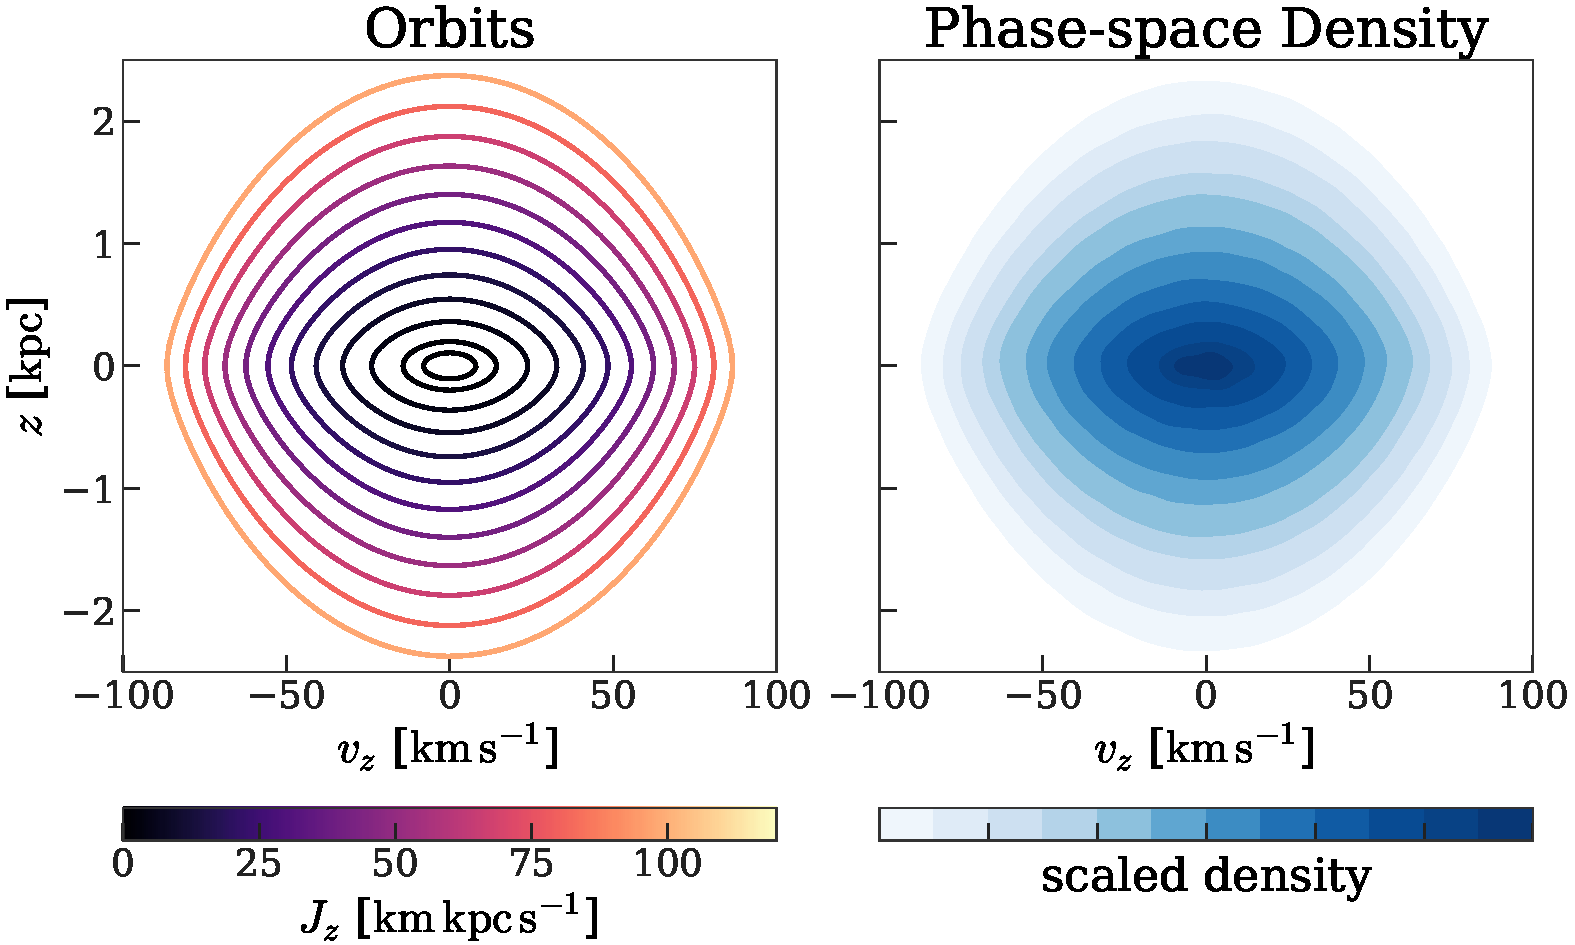
\includegraphics[width=0.8\textwidth]{illustrate-zvz.pdf}
\end{center}
\caption{%
TODO
\label{fig:zvz}
}
\end{figure}

Orbits in the vertical coordinate in a Galactic disk embedded in a dark matter halo are
more complex.
Figure~\ref{fig:zvz} is an illustration that shows several sample orbits with different
values of the vertical action (spaced uniformly in $\sqrt{J_z}$), all with $J_R=0$ and
the same $J_\phi$ in a two-component galaxy model consisting of a Miyamoyo--Nagai disk
component \citep{Miyamoto:1975} and a Navarro--Frenk--White (NFW) halo component
\citep{NFW:1996} with parameters chosen to roughly match a Milky Way-like configuration
(but this potential model is only used for illustrative purposes).
For smaller values of the vertical action, orbits are close to elliptical in shape with
a frequency (axis ratio) that changes with action.
For orbits with larger vertical action (i.e. for orbits that feel the influence of the
dark matter halo), the orbital trajectory shapes become more ``diamond''-like.
To describe the density distribution resulting from a mixture of stars drawn from




\begin{align}
    \theta_z' &= \arctan{\left(\frac{z}{v_z} \, \omega_0 \right)} \\
    r_z &= r_z' \, \left[1 + \sum_m \epsilon_m(r_z') \, \cos{\left(m\,\theta_z'\right)}\right]
\end{align}

Choice of $n(r_z)$ or $f(r_z)$, choice of $\epsilon_m(r_z')$.

\begin{align}
    J_z &= \frac{2}{\pi} \, \int_0^{\pi/2} \dd \theta_z' \, v_z(\theta_z')
        \, \left|\frac{\dd r_z'}{\dd \theta_z'}\right| \\
    T_z &= 4 \, \int_0^{\pi/2} \frac{\dd \theta_z'}{v_z(\theta_z')}
        \, \left|\frac{\dd r_z'}{\dd \theta_z'}\right| \quad
\end{align}
where
\begin{equation}
    v_z(\theta_z') = r_z'(r_z, \theta_z') \, \cos{(\theta_z')}
\end{equation}


\section{Data} \label{sec:data}


\section{Results} \label{sec:results}


\section{Discussion} \label{sec:discussion}


\section{Conclusions} \label{sec:conclusions}


\begin{acknowledgements}

It is a pleasure to thank ...

% Funding for the Sloan Digital Sky Survey IV has been provided by the Alfred P.
% Sloan Foundation, the U.S. Department of Energy Office of Science, and the
% Participating Institutions. SDSS-IV acknowledges support and resources from the
% Center for High-Performance Computing at the University of Utah. The SDSS web
% site is www.sdss.org.

% SDSS-IV is managed by the Astrophysical Research Consortium for the
% Participating Institutions of the SDSS Collaboration including the Brazilian
% Participation Group, the Carnegie Institution for Science, Carnegie Mellon
% University, the Chilean Participation Group, the French Participation Group,
% Harvard-Smithsonian Center for Astrophysics, Instituto de Astrof\'isica de
% Canarias, The Johns Hopkins University, Kavli Institute for the Physics and
% Mathematics of the Universe (IPMU) / University of Tokyo, Lawrence Berkeley
% National Laboratory, Leibniz Institut f\"ur Astrophysik Potsdam (AIP),
% Max-Planck-Institut f\"ur Astronomie (MPIA Heidelberg), Max-Planck-Institut
% f\"ur Astrophysik (MPA Garching), Max-Planck-Institut f\"ur Extraterrestrische
% Physik (MPE), National Astronomical Observatories of China, New Mexico State
% University, New York University, University of Notre Dame, Observat\'ario
% Nacional / MCTI, The Ohio State University, Pennsylvania State University,
% Shanghai Astronomical Observatory, United Kingdom Participation Group,
% Universidad Nacional Aut\'onoma de M\'exico, University of Arizona, University
% of Colorado Boulder, University of Oxford, University of Portsmouth, University
% of Utah, University of Virginia, University of Washington, University of
% Wisconsin, Vanderbilt University, and Yale University.

This work has made use of data from the European Space Agency (ESA) mission
{\it Gaia} (\url{https://www.cosmos.esa.int/gaia}), processed by the {\it Gaia}
Data Processing and Analysis Consortium (DPAC,
\url{https://www.cosmos.esa.int/web/gaia/dpac/consortium}). Funding for the DPAC
has been provided by national institutions, in particular the institutions
participating in the {\it Gaia} Multilateral Agreement.

\end{acknowledgements}

\software{
    Astropy \citep{astropy:2013, astropy:2018, astropy:2022},
    gala \citep{gala},
    IPython \citep{ipython},
    numpy \citep{numpy},
    % pymc3 \citep{Salvatier2016},
    % schwimmbad \citep{schwimmbad:2017},
    scipy \citep{scipy}.
}

\bibliographystyle{aasjournal}
\bibliography{empirical-af}

\end{document}
